\documentclass{article}

% Use the Cactus ThornGuide style file
% (Automatically used from Cactus distribution, if you have a
%  thorn without the Cactus Flesh download this from the Cactus
%  homepage at www.cactuscode.org)
\usepackage{../../../../doc/latex/cactus}

\begin{document}

\title{PUGH}
\author{The Cactus Team\\{\tt cactusmaint@cactuscode.org}}
\date{$ $Date$ $}

\maketitle

% Do not delete next line
% START CACTUS THORNGUIDE

\begin{abstract}
The default unigrid driver for Cactus for both multiprocessor and single process runs, handling grid variables and communications.
\end{abstract}

\section{Description}

PUGH can create, handle and communicate grid scalars, arrays and functions
in 1, 2 or 3-dimensions.

\section{Compilation}

PUGH can be compiled with or without MPI. Compiling without MPI results
in an executable which can only be used on a single processor, compiling
with MPI leads to an executable which can be used with either single or
multiple processors.
(Section~\ref{pugh_understanding} describes how you can tell if your
executable has been compiled with or without MPI).

For configuring with MPI, see the Cactus User's Guide.

\section{Grid Size}

The number of grid points used for a simulation can be set in PUGH either
globally (that is, the total number of points across all processors), or
locally (that is, the number of points on each processor).

To set the global size of a N-D grid to be 40 grid points in each direction use

\begin{verbatim}
  PUGH::global_nsize = 40
\end{verbatim}

To set the global size of a 2D grid to be $40\times 20$ use

\begin{verbatim}
  PUGH::global_nx = 40
  PUGH::global_ny = 20
\end{verbatim}

To set the local size of a 2D grid to be $40\times 20$ on each processor, use

\begin{verbatim}
  PUGH::local_nx = 40
  PUGH::local_ny = 20
\end{verbatim}


\section{Periodic Boundary Conditions}

PUGH can implement periodic boundary conditions during the synchronization
of grid functions. Although this may at first seem a little confusing, and
unlike the usual use of boundary conditions which are directly called from
evolution routines, it is the most efficient and natural place for periodic
boundary conditions.

PUGH applies periodic conditions by simply communicating the appropriate
ghostzones between ``end'' processors. For example, for a 1D domain with two
ghostzones, split across two processors, Figure~\ref{pugh::fig1} shows the implementation of periodic boundary conditions.

\begin{figure}[ht]
\begin{center}
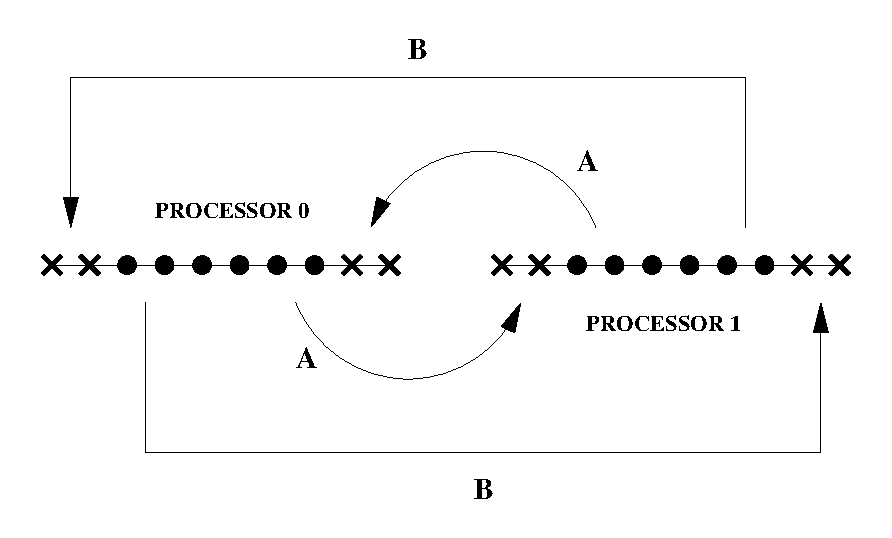
\includegraphics[angle=0,width=8cm]{periodic}
\end{center}
\caption[]{Implementation of periodic boundary conditions for a 1D domain, with two ghostzones, split across two processors. The lines labelled {\bf A} show the {\it standard} communications during synchronisation, the lines labelled
{\bf B} show the additional communications for periodic boundary conditions.}
\label{pugh::fig1}
\end{figure}

Periodic boundary conditions are applied to all grid functions, by default
they are applied in all directions, although this behaviour can be customised
to switch them off in given directions.

By default, no periodic boundary conditions are applied. To apply periodic boundary conditions in all directions, set

\begin{verbatim}
  PUGH::periodic = "yes"
\end{verbatim}

To apply periodic boundary conditions in just the x- and y- directions in
a 3 dimensional domain, use

\begin{verbatim}
  PUGH::periodic = "yes"
  PUGH::periodic_z = "no"
\end{verbatim}


\section{Processor Decomposition}

%\section{Load Balancing}
By default PUGH will distribute the computational grid evenly across
all processors (as in Figure~\ref{pugh::fig2}a). This may not be
efficient if there is a different computational load on different
processors, or for example for a simulation distributed across
processors with different per-processor performance.

\begin{figure}[ht]
\begin{center}
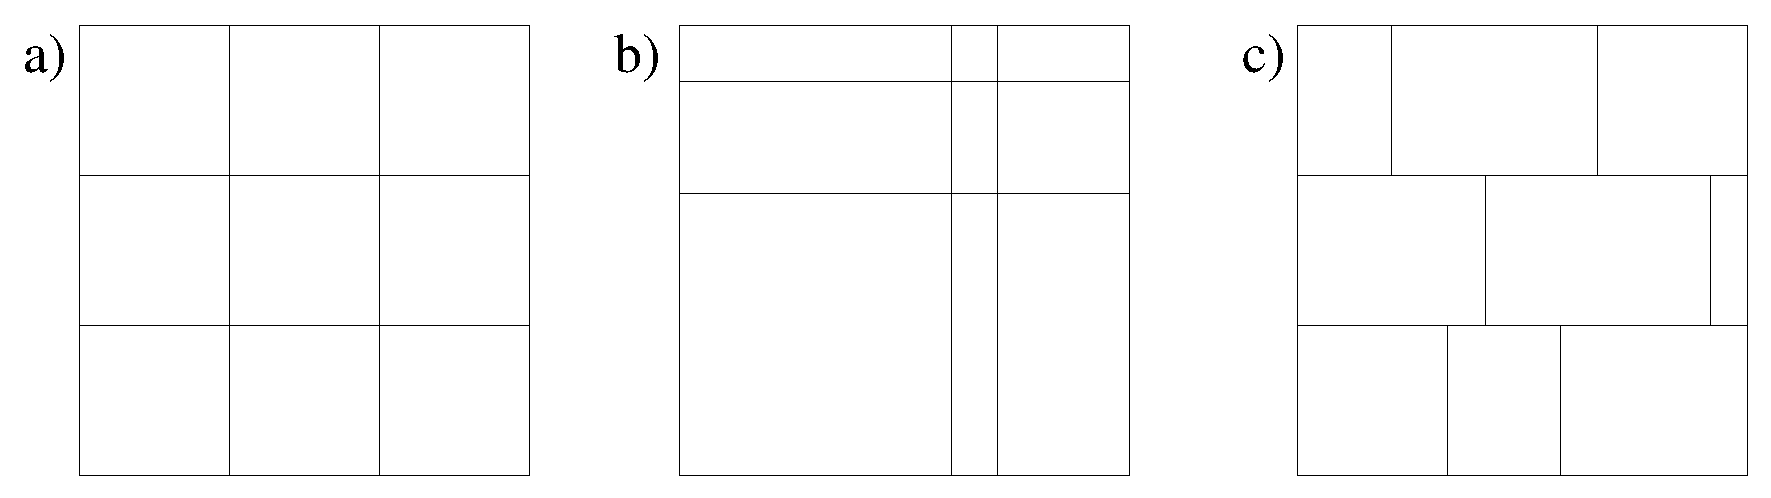
\includegraphics[angle=0,width=12cm]{Partitioning}
\end{center}
\caption[]{Partitioning of the computational grid across processors, Figure~a) is the default type of partition used by {\tt PUGH}, Figure~b) can be set
manually, and Figure~c) is not possible with {\tt PUGH}}
\label{pugh::fig2}
\end{figure}

The computational grid can be manually partitioned in each direction
in a regularly way as in Figure~\ref{pugh::fig2}b.

The computational grid can be manually distributed using PUGH's
string parameters \verb!partition_[1d_x|2d_x|2d_y|3d_x|3d_y|3d_z]!.
To manually specify the load distribution, set {\tt PUGH::partition = "manual"}
and then, depending on the grid dimension, set the remaining
parameters to distribute the load in each direction. Note that for
this you need to know apriori the processor decomposition.

The decomposition is easiest to explain with a simple example:
to distribute a 30-cubed grid across 4 processors (decomposed as $2 \times 1
\times 2$, with processors 0 and 2 performing twice as fast as processors 1
and 3) as:

\begin{tabular}{cc}
proc 2: $20 \times 30 \times 15$ & proc 3: $10 \times 30 \times 15$ \\
proc 0: $20 \times 30 \times 15$ & proc 1: $10 \times 30 \times 15$ \\
\end{tabular}

you would use the following topology and partition parameter settings:

\begin{verbatim}
  # the overall grid size
  PUGH::global_nsize = 30

  # processor topology
  PUGH::processor_topology      = manual
  PUGH::processor_topology_3d_x = 2
  PUGH::processor_topology_3d_y = 1
  PUGH::processor_topology_3d_z = 2     # redundant

  # grid partitioning
  PUGH::partition      = "manual"
  PUGH::partition_3d_x = "20 10"
\end{verbatim}

Each partition parameter lists the number of grid points for every processor
in that direction, with the numbers delimited by any non-digit characters.
Note that an empty string for a direction (which is the default value for
the partition parameters) will apply the automatic distribution. That's why
it is not necessary to set \verb|PUGH::partition_3d_y = "30"| or
\verb|PUGH::partition_3d_z = "15 15"| in the parameter file.

Because the previous automatic distribution gave problems in some
cases (e.g.\ very long box in one, but short in other directions),
there is now an improved algorithm that tries to do a better job in
decomposing the grid evenly to the processors.  However, it can fail
in certain situations, in which it is gracefully falling back to the
previous (\verb|"automatic_old"|) giving a warning.  Note that, if one
or more of the parameters \verb|PUGH::processor_topology_3d_*| or
\verb|PUGH::partition_3d_*| are set, this mode automatically falls back to
\verb|"automatic_old"| without warning.

\section{Understanding PUGH Output}

\label{pugh_understanding}

PUGH reports information about the processor decomposition to standard output
at the start of a job. This section describes how to interpret that output.

\vskip .3cm

\noindent
{\bf Single Processor (no MPI)}

\begin{itemize}

\item{\bf Type of evolution}

If an executable has been compiled for only single processor use
(without MPI), the first thing which PUGH reports is this fact:

{\tt INFO (PUGH): Single processor evolution}

\end{itemize}


\vskip .3cm

\noindent
{\bf Multiple Processor (with MPI)}



\vskip .3cm

\begin{itemize}

\item{\bf Type of evolution}

If an executable has been compiled using MPI, the first thing which
PUGH reports is this fact, together with the number of processors
being used:

{\tt INFO (PUGH): MPI Evolution on 3 processors}


\item{\bf Maximum load skew}

The maximum load skew describes the variance in the number of gridpoints on
each processor, and is defined by

$$\mbox{Max Skew} = 100 \;\;\frac{\mbox{Max Points}- \mbox{Min Points}}{\mbox{Average Points}} $$

For most purposes, the maximum skew should ideally be close to zero,
however if your simulation has a different load at different grid
points, or if you are running across processors with different
properties, the optimal skew could be quite different.

By default, PUGH tries to minize the skew in gridpoints, however this may
be overriden by performing the load balancing manually.

\end{itemize}

\section{Useful Parameters}

There are several parameters in PUGH which are useful for debugging and
optimisation:

\begin{Lentry}

\item[{\tt PUGH::enable\_all\_storage}]

Enables storage for all grid variables (that is, not only
those set in a thorn's {\tt schedule.ccl} file). Try this parameter
if you are getting segmentation faults.  If enabling all storage
removes the problem, it most likely means that you are accessing
a grid variable (probably in a Fortran thorn) for which storage
has not been set.

\item[{\tt PUGH::initialise\_memory}]

By default, when PUGH allocates storage for a grid variable it
does not initialise its elements. If you access an
uninitialised variable on some platforms you will get a
segmentation fault (and in general you will see erratic
behaviour). This parameter can be used to initialise all
elements to zero, if this removes your segmentation fault you
can then track down the cause of the problem by using the same
parameter to initialize all elements to NaNs and then track
them with the thorn {\tt CactusUtils/NaNChecker}.

   Note that it isn't recommended to simply use this parameter to
initialise all elements to zero, instead we recommend you to
set all variables to their correct values before using them.

\item[{\tt PUGH::storage\_verbose}]

This parameter can be set to print out the number of grid variables
which have storage allocated at each iteration, and the total
size of the storage allocated by Cactus. Note that this total
does not include storage allocated independently in thorns.

\item[{\tt PUGH::timer\_output}]

This parameter can be set to provide the time spent communicating
variables between processors.

\end{Lentry}

% Do not delete next line
% END CACTUS THORNGUIDE

\end{document}
